\documentclass[dvipdfmx]{jsarticle}
\usepackage{graphics}
\usepackage{amsmath}
\usepackage{amssymb}
\usepackage{amsthm}
\usepackage{mathtools}
\usepackage{ascmac}
\usepackage{bm}
\usepackage{url}
\usepackage{txfonts}
\usepackage{tikz}
% \usepackage{docmute}    %パッケージのダウンロードが必要
\usepackage{tikz}
\usetikzlibrary{calc}
\usetikzlibrary{intersections}



% \usepackage[dvipdfmx]{hyperref}
% \usepackage{pxjahyper}

\newcommand{\mmm}{\hspace{3mm}}
\newcommand{\veczero}{$\vec{0}$}
\newcommand{\veca}{$\vec{a}$}
\newcommand{\vecb}{$\vec{b}$}
\newcommand{\veco}{$\vec{o}$}
\newcommand{\vecx}{$\vec{x}$}
\newcommand{\vecy}{$\vec{y}$}
\newcommand{\vecz}{$\vec{z}$}
\newcommand{\vecrm}[1]{$\overrightarrow{\mathrm{ #1 }}$}
\newcommand{\vecins}[1]{$\vec{#1}$}
\newcommand{\mathins}[1]{${#1}$}


\begin{document}
    \section{ベクトルと図形での問題}
    この章で理解できる問題は以下の通りだ.
    \begin{itemize}
        \item 点の位置関係(同一直線上)
        \item 点の位置関係(同一平面上)
        \item チェバの定理・メネラウスの定理
        % \item 三角形の五心(外心,内心,重心)
        % \item 点,直線,平面の表現
        \item 図形の性質のベクトルによる確認
    \end{itemize}

    \subsection{点の位置関係(同一直線上)}
    \begin{itembox}[l]{問題}
        以下の平行六面体\footnote{向かい合った面が合同な平行四辺形となってる立体を平行六面体という.平行六面体では向かい合った面が平行となる.}において,\mathins{\bigtriangleup\mathrm{ABC}}の重心を\mathins{\mathrm{G}},\mathins{\bigtriangleup\mathrm{PQR}}の重心を\mathins{\mathrm{G}'}とする.このとき,3点\mathins{\mathrm{O},\mathrm{G},\mathrm{G}'}が一直線上にあることを証明せよ.
        %立方体の図

        \begin{centering}
            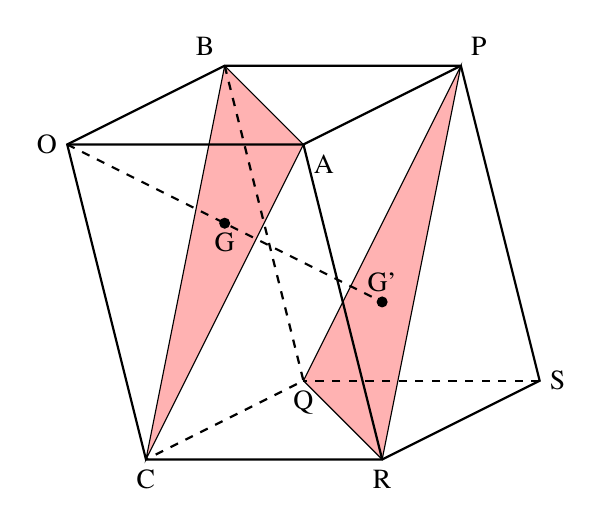
\begin{tikzpicture}
                \coordinate (o) at (0,0);
                \coordinate (a) at (3,0);
                \coordinate (b) at (2,1);
                \coordinate (p) at (5,1);
                \coordinate (c) at (1,-4);
                \coordinate (r) at (4,-4);
                \coordinate (q) at (3,-3);
                \coordinate (s) at (6,-3);

                \filldraw[fill=red!30,draw=black](b)--(a)--(c)--cycle;
                \filldraw[fill=red!30,draw=black](p)--(q)--(r)--cycle;

                \coordinate (g1) at ($0.3333*(a)+0.3333*(b)+0.3333*(c)$);
                \coordinate (g2) at ($0.3333*(p)+0.3333*(q)+0.3333*(r)$);
                \fill (g1)node[below]{G}  circle (2pt);
                \fill (g2)node[above]{G'} circle  (2pt);
                \draw[thick,dashed](o)--(g1)--(g2);

                % 平行六面体の線
                \draw[thick](o)node[left]{O}--(b)node[above left]{B}--(p)node[above right]{P}--(s)node[right]{S}--(r)node[below]{R}--(c)node[below]{C}--cycle;
                \draw[thick](o)--(a)node[below right]{A}--(p);
                \draw[thick](a)--(r);
                \draw[thick,dashed](b)--(q)node[below]{Q}--(c);
                \draw[thick,dashed](s)--(q);

            \end{tikzpicture}
            % \figcaption{立体\label{tikz_question_2_1_ritai}}


        \end{centering}
    \end{itembox}

    Oの基準とする位置ベクトルを置くことで計算を簡単にする.位置ベクトルを次のようにおく.
    \[
    \mathrm{A}(\vec{a}),\mmm\mathrm{B}(\vec{b}),\mmm\mathrm{C}(\vec{c}),\mmm\mathrm{P}(\vec{p}),\mmm\mathrm{Q}(\vec{q}),\mmm\mathrm{R}(\vec{r})
    \]
    平行六面体の図形的な条件より
    \[
    \vec{p}=\vec{a}+\vec{b},\mmm\vec{q}=\vec{b}+\vec{c},\mmm\vec{r}=\vec{c}+\vec{a}
    \]
    がわかる.ここから重心の重心の位置ベクトルを計算する.
    \begin{eqnarray*}
        \vec{g}&=&\frac{1}{3}(\vec{a}+\vec{b}+\vec{c})\\
        \vec{g'}&=&\frac{1}{3}(\vec{p}+\vec{q}+\vec{r})=\frac{2}{3}(\vec{a}+\vec{b}+\vec{c})
    \end{eqnarray*}
    すると\vecrm{OG}と\vecrm{OG'}には次の関係が成立する.
    \[
    \overrightarrow{\mathrm{OG}}=\frac{1}{2}\overrightarrow{\mathrm{OG'}}
    \]
    したがって3点\mathins{\mathrm{O},\mathrm{G},\mathrm{G}'}は一直線上に存在する.

    \subsection{点の位置関係(同一平面上)}
    \begin{itembox}[l]{問題}
        3点\mathins{\mathrm{A}(-1,2,1),\mathrm{B}(2,-2,3),\mathrm{C}(2,4,-1)}の定める平面ABC上に点\mathins{\mathrm{P}(x,3,1)}があるとき,\mathins{x}の値を求めよ.
    \end{itembox}


    これはA,B,Cのうちの1つを基準としたベクトルを考えればいい.基準をAとして次のベクトルをとる.
    \[
    \overrightarrow{\mathrm{{AB}}}=(3,-4,4),\mmm\overrightarrow{\mathrm{AC}}=(3,2,0),
    \mmm\overrightarrow{\mathrm{AP}}=(x+1,1,2)
    \]
    となる.Pが平面ABC上にあることから
    \[
    \overrightarrow{\mathrm{AP}}=s\overrightarrow{\mathrm{{AB}}}+t\overrightarrow{\mathrm{AC}}\mmm (s,t\in \mathbb{R})
    \]
    である.成分表示の結果を代入することで
    \begin{eqnarray*}
        (x+1,1,2)&=&s(3,-4,4)+t(3,2,0)\\
        &=&(3s+3t,-4s+2t,4s)
    \end{eqnarray*}
    を得る.y成分とz成分に注目すると
    \[
    s=\frac{1}{2},\mmm t=\frac{3}{2}
    \]
    がわかる.あとはx成分に注目することで
    \[
    x=5
    \]
    という結論を得る.

    \begin{figure}[htbp]\centering
        \begin{tikzpicture}
            % 直交座標の規定を定義
            \coordinate (o) at (0,0);
            \coordinate (x) at (0:1);
            \coordinate (y) at (220:1);
            \coordinate (z) at (90:1);

            % 軸を描く
            \draw[->] (o)--($5*(x)$)node[right]{\mathins{x}};
            \draw[->] (o)--($5*(y)$)node[below left]{\mathins{y}};
            \draw[->] (o)--($5*(z)$)node[above]{\mathins{z}};
            \draw (o)--($-5*(x)$);
            \draw (o)--($-5*(y)$);
            \draw (o)--($-5*(z)$);

            \coordinate (a) at ($-1*(x)+2*(y)+1*(z)$);
            \coordinate (b) at ($2*(x)-2*(y)+3*(z)$);
            \coordinate (c) at ($2*(x)+4*(y)-1*(z)$);
            \coordinate (p) at ($5*(x)+3*(y)+1*(z)$);

            \fill (a)node[below left]{A} circle (2pt);
            \fill (b)node[above]{B} circle (2pt);
            \fill (c)node[below left]{C} circle (2pt);
            \fill (p)node[below left]{P} circle (2pt);


            \draw[ultra thick,->,red](a)--(b);
            \draw[ultra thick,->,red](a)--(c);
            \draw[ultra thick,->,blue](a)--(p);

        \end{tikzpicture}
        \caption{イメージ図}
        \label{tikz_question_2_2_kaito}
    \end{figure}





    \subsection{チェバの定理・メネラウスの定理}
    \begin{itembox}[l]{問題}
        \mathins{\bigtriangleup \mathrm{OAB}}
        に対して,辺OAを\mathins{1:3}に内分する点をP,
        辺OBを\mathins{2:3}に内分する点をQとする.
        線分AQと線分BPの交点Gとしたときのベクトル\mathins{\overrightarrow{\mathrm{OG}}}を
        \mathins{\overrightarrow{\mathrm{OA}},\overrightarrow{\mathrm{OB}}}を用いて表せ.また,\mathins{\overrightarrow{\mathrm{OG}}}を延長して線分ABとの交点をTとしたとき,\mathins{\overrightarrow{\mathrm{T}}}を
        \mathins{\overrightarrow{\mathrm{OA}},\overrightarrow{\mathrm{OB}}}を用いて表せ.

        \begin{centering}

            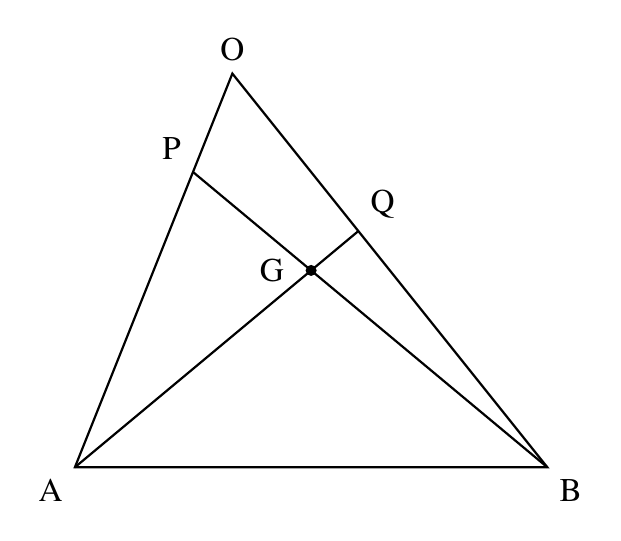
\begin{tikzpicture}\large
                \coordinate (o) at (0,0);
                \coordinate (a) at (-2,-5);
                \coordinate (b) at (4,-5);
                \draw[thick] (o)node[above]{O}--(a)node[below left]{A}--(b)node[below right]{B}--cycle;
                \draw[thick,name path=aq] (a)--($0.4*(b)$)node[above right]{Q};
                \draw[thick,name path=bp] (b)--($0.25*(a)$)node[above left]{P};
                \fill[name intersections={of=aq and bp,by={g}}](g)node[left=2mm]{G} circle (2pt);

                % \fill[red]($2/6*(a) + 2/3*(b)$) circle(2pt);
            \end{tikzpicture}

        \end{centering}

    \end{itembox}

    その気になれば,メネラウスの定理やチェバの定理を使うことで与えられた線分の長さの比から答えを導くことができる.しかし,ここではベクトルの一意性を用いて答えを求める.まず線分の比を自分で与える\footnote{線分AQ,BPに対して,その内分点Gに関する比を与える.与え方は自由だ.}.

    \begin{align*}
        \mathrm{AG}:\mathrm{GQ}&=s:1-s\\
        \mathrm{BG}:\mathrm{GP}&= t:1-t
    \end{align*}
    と与える.すると,
    \begin{align*}
        \overrightarrow{\mathrm{OG}}&=(1-s) \overrightarrow{\mathrm{OA}}
        +s \overrightarrow{\mathrm{OQ}}\\
        &= (1-s) \overrightarrow{\mathrm{OA}}
        + \frac{2}{5}s \overrightarrow{\mathrm{OB}}\\
        \overrightarrow{\mathrm{OG}} &= t \overrightarrow{\mathrm{OP}}
        +(1-t)\overrightarrow{\mathrm{OB}}\\
        &= \frac{1}{4}t \overrightarrow{\mathrm{OA}}
        +(1-t)\overrightarrow{\mathrm{OB}}
    \end{align*}
    となる.

    このように同一のベクトル \(\overrightarrow{\mathrm{OG}}\)が2通りの表現で表されている.また, \(\overrightarrow{\mathrm{OA}},\overrightarrow{\mathrm{OB}}\)は一次独立である.したがって,ベクトルの一意性より次の連立方程式を得る.
    \[
    \begin{cases}
        \displaystyle 1-s=\frac{1}{4}t\\
        \displaystyle\frac{2}{5}s=1-t
    \end{cases}
    \]
    連立方程式を解くと
    \[
    s=\frac{5}{6},\quad t=\frac{2}{3}
    \]
    となる.したがって
    \[
    \overrightarrow{\mathrm{OG}} = \frac{1}{6}\overrightarrow{\mathrm{OA}}+\frac{1}{3}\overrightarrow{\mathrm{{OB}}}
    \]
    となる.これで前半を答えたことになる.自ら線分の比を与え,それを連立方程式の利用によって求める.

    次は後半の部分で, \(OG\)を延長することを考える.このとき,3点O,G,Tは同一直線上にあることから,
    \[
    \overrightarrow{\mathrm{OT}}=k \overrightarrow{\mathrm{{OG}}}\qquad (k\text{は実数})
    \]
    とすることができる.この \(k\)を求めることができればよい.さらに条件として,3点A,T,Bは同一直線上にあるので,
    \[
    \overrightarrow{\mathrm{OT}}=x \overrightarrow{\mathrm{OA}}+y\overrightarrow{\mathrm{OB}}
    \]
    とすることができた場合,係数の和が \(x+y=1\)となる.したがって,
    \begin{align*}
        k\left(\frac{1}{6}+\frac{1}{3}\right)&=1\\
        &\Rightarrow k= 2\\
        \therefore \overrightarrow{\mathrm{OT}}&=\frac{1}{3}\overrightarrow{\mathrm{OA}}
        +\frac{2}{3}\overrightarrow{\mathrm{OB}}
    \end{align*}

    \subsection{図形の性質のベクトルによる確認}
    ベクトルの問題では数Aで学習した図形の持つ性質をベクトルを用いて再確認させるようなものがよくある.ある意味で当然なことを示すのだが,これが難しい場合がある.大抵,問題で与えられた図形の持つもともとの条件を忘れることが理由なので,落ち着いて問題にあたりたい.
    \begin{itembox}[l]{問題}
        \begin{enumerate}
            \item 正四面体において,交点を持たない2本の辺は垂直であることを示せ.
            \item 四面体ABCDにおいて, \(\mathrm{AC}\perp \mathrm{BD}\)ならば,
            \[
            \mathrm{AD}^2+\mathrm{BC}^2=\mathrm{AB}^2+\mathrm{CD}^2
            \]
            が成立することを示せ.
        \end{enumerate}
    \end{itembox}

    1問目は,つかみどころのないような問題文にしてみた.問題の様子を図\ref{tikz_sei_4_mentai}にする.例えば,赤線としてある2本の辺が交点を持たない辺の組である.正四面体において,この赤線の辺の組は垂直であるのだ.
    \begin{figure}[htbp]\centering
        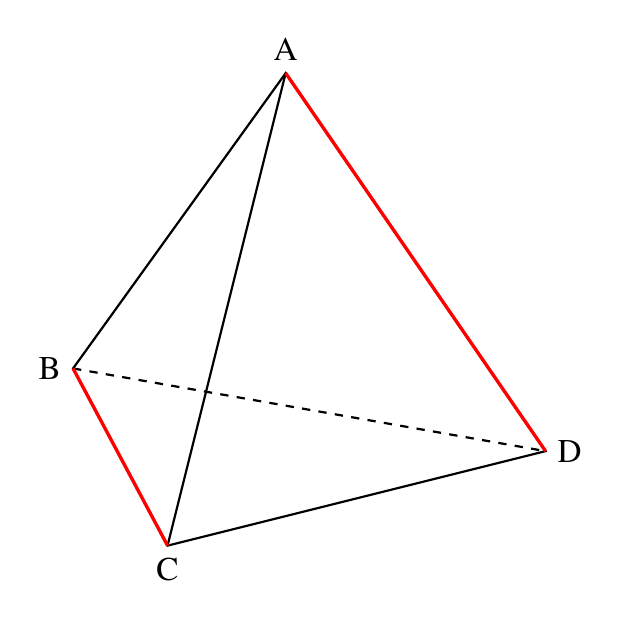
\begin{tikzpicture}[scale=1.5]\large
            \coordinate (a) at (1,4);
            \coordinate (b) at (-0.8,1.5);
            \coordinate (c) at (0,0);
            \coordinate (d) at (3.2,0.8);
            \draw[thick](a)node[above]{A}--(b)node[left]{B}--(c)node[below]{C}--(d)node[right]{D}--cycle;
            \draw[thick](a)--(c);
            \draw[thick,dashed](b)--(d);
            \draw[red,very thick](b)--(c);
            \draw[red,very thick](a)--(d);
        \end{tikzpicture}
        \caption{正四面体}
        \label{tikz_sei_4_mentai}
    \end{figure}

    解法の手順としては,正四面体の頂点のどれかを定点とした位置ベクトルを置くことから始まる.また,頂点の名前は自由における状態であるということは,1つの辺の組さえ証明してしまえば,図形の対称性から残りは自明となることを利用する.証明問題なので,厳密に解答する.

    \begin{proof}
        図\ref{tikz_sei_4_mentai}の正四面体において,点Aを始点とした位置ベクトルを考え,残りの3点は位置ベクトルで \(\vec{b},\vec{c},\vec{d}\)と表すことにする.正四面体であるという条件から,すべての辺の長さは等しく,また,隣り合った2辺のなす角は60度である.したがって,
        \[
        \vec{b}\cdot\vec{c}=\vec{c}\cdot\vec{d}=\vec{d}\cdot\vec{b}
        \]
        である.

        これを用いると,
        \begin{align*}
            \vec{d}\cdot(\vec{b}-\vec{c})&= \vec{d}\cdot\vec{b}-\vec{d}\cdot\vec{c}\\
            &=0\\
            \therefore \mathrm{AD}&\perp \mathrm{BC}
        \end{align*}
        と分かる.つまり,交点を持たない2本の辺の組の1つであるAD,BCで題意を示したことになる.さらに,図形の対称性より,同様の議論を繰り返すことで,すべての交点を持たない2本の辺の組で題意を示すことができる.

    \end{proof}

    2問目は立体の図形的な情報を辺の長さという数値の情報に変換する問題だ.図\ref{tikz_simentai}の赤い部分が垂直であるのが条件である\footnote{図の使いまわし,すみません.}.

    \begin{figure}[htbp]\centering
        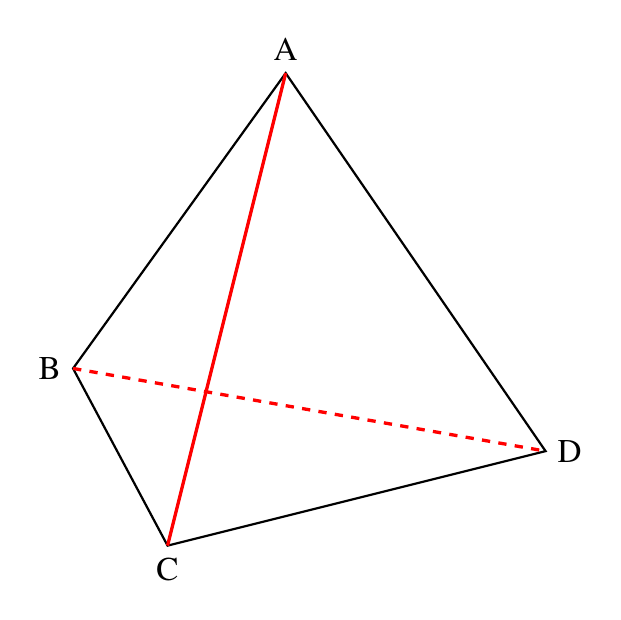
\begin{tikzpicture}[scale=1.5]\large
            \coordinate (a) at (1,4);
            \coordinate (b) at (-0.8,1.5);
            \coordinate (c) at (0,0);
            \coordinate (d) at (3.2,0.8);
            \draw[thick](a)node[above]{A}--(b)node[left]{B}--(c)node[below]{C}--(d)node[right]{D}--cycle;
            \draw[thick](a)--(c);
            \draw[red ,very thick,dashed](b)--(d);
            \draw[red,very thick](a)--(c);
        \end{tikzpicture}
        \caption{正四面体}
        \label{tikz_simentai}
    \end{figure}

    \begin{proof}

        図\ref{tikz_simentai}の正四面体において,点Aを始点とした位置ベクトルを考え,残りの3点は位置ベクトルで \(\vec{b},\vec{c},\vec{d}\)と表すことにする.
        問題の条件より \(\mathrm{AC}\perp \mathrm{BD}\)なので,
        \begin{align*}
            \vec{c}\cdot (\vec{d}-\vec{b})&= \vec{c}\cdot\vec{d}-\vec{c}\cdot\vec{b}\\
            &=0\\
            \therefore \vec{c}\cdot\vec{b}&=\vec{c}\cdot\vec{d}
        \end{align*}

        さて,ここで示すべき式の左辺をベクトルで計算する.
        \begin{align*}
            (\text{左辺})&=|\vec{d}|^2 +|\vec{c}-\vec{b}|^2\\
            &=|\vec{b}|^2 +|\vec{c}|^2 +|\vec{d}|^2 -2\vec{c}\cdot\vec{b}
        \end{align*}
        同様に右辺もベクトルで計算する.
        \begin{align*}
            (\text{右辺})&=|\vec{b}|^2+|\vec{d}-\vec{c}|^2\\
            &=|\vec{b}|^2 +|\vec{c}|^2 +|\vec{d}|^2 -2\vec{c}\cdot\vec{d}
        \end{align*}
        \(\vec{c}\cdot\vec{b}=\vec{c}\cdot\vec{d}\)より \((\text{左辺})=(\text{右辺})\)
    \end{proof}

    






\end{document}
